\documentclass[sigconf]{acmart}

\usepackage{hyperref}

\usepackage{endfloat}
\renewcommand{\efloatseparator}{\mbox{}} % no new page between figures

\usepackage{booktabs} % For formal tables

\settopmatter{printacmref=false} % Removes citation information below abstract
\renewcommand\footnotetextcopyrightpermission[1]{} % removes footnote with conference information in first column
\pagestyle{plain} % removes running headers

\begin{document}
\title{Big Data and Artificial Intelligence Solutions for in Home, Community and Territory Security}


\author{Ashok Reddy Singam}
\orcid{HID337}
\affiliation{%
  \institution{Indiana University}
  \streetaddress{711 N Park Ave}
  \city{Bloomington} 
  \state{Indiana} 
  \postcode{47408}
}
\email{asingam@iu.edu}

\author{Anil Ravi}
\orcid{HID333}
\affiliation{%
  \institution{Indiana University}
  \streetaddress{711 N Park Ave}
  \city{Bloomington} 
  \state{Indiana} 
  \postcode{47408}
}
\email{anilravi@iu.edu}

\begin{abstract}
Anti-social activities became the most significant threat to national security because of their potential to bring massive damage to our homes, public infrastructure, economy, and people. The existing systems and methods haven’t reached the level of sophistication to be able to consolidate the relevant data from variety of sources and demographics. Video surveillance of residential, commercial, military, and other restricted locations have been in practice since many years using various available technologies. Depending on the level of security, the data has been processed by data mining and/or big data analytics to take decisions by various personal, agencies and governments. However, the limitations of data collection, data mining and adoption of intelligence led to ineffective systems which are not predictive as they should be. With the advent of technologies, it possible to integrate the video, audio and social media data of targeted regions (homes, public places and extended areas) for security analysis. Such systems can use advanced statistical methods, classification algorithms and machine learning algorithms to predict and prevent the threats based on the severity probability.

\end{abstract}

\keywords{i523, HID333, HID337, Artificial Intelligence, Natural Language Processing (NLP), Machine Learning, Micro Drone}

\maketitle

\section{Introduction}
As per the book “Intelligence and Security Informatics”[1], it is widely believed that information technology will play an indispensable role in making the world safer by supporting intelligence and knowledge discovery through collecting, processing, analyzing, and utilizing terrorism- and crime-related data. Social network analysis (SNA) has been widely explored to support intelligence and law enforcement agencies in investigating the terrorist and criminal social networks. It is valuable in identifying terrorists, suspect subgroups, and their communication patterns.

However, in the present world, the systems are disparately processing the data and the decisions/conclusions are being made without considering from multiple dimensions. The large corporations, nations, and intelligence agencies are using their individual systems but not taking integrated approach to solve the problems in their entirety. This could be due to political and economic interests of individuals, corporations and nations.

Analyzing the individual human behaviors, interactions, transactions, and actions is the key element in identifying the potential threat in advance. Generating and analyzing such data from individual homes and extending the concept to larger groups is the idea behind this research.

It is quite feasible to collect the data from individual homes and roll up to the communities, cities and then to the nations across the world. Since this involves with the personal data from people directly, it is required to follow privacy-preservation policies and methods enforced by local/national governments and law enforcement agencies. By accessing the lowest level of data of individuals’ video, voice, social media and other business transactional data would allow to characterize, analyze and assess the people behaviors and motives which can be maintained and processed as needed by Big Data systems. These systems are very complex in nature due to the variety, volume and velocity of the data, where the Big Data technologies will play a significant role in realizing them. In addition to data collection and mining, if artificial intelligence is applied to analyze and evaluate the data then the crime prediction and prevention would be feasible.

In order to realize such systems, one would need several technologies and sub-systems in various layers to effectively collect, transfer, mining, learning and analyze the data. In the following sections, it has been described some of the technologies/sub-systems that can be used to achieve the objectives of proposed conceptual model.

The discussion here consists of reviewing the available papers/systems related to security informatics and understanding the technologies and methods used. The gaps perceived in the review are attempted to solve by proposing a new concept. The remainder of this discussion is organized as follows: Section 2 provides a set of sub-systems and use of them in the proposed framework. Section 3 gives an overview community/city security using conceptual model. Finally, section 4 concludes this proposal.


\subsection{Contemporary Security Systems}

The present security systems used by households are static cameras used at a fixed location inside or outside the house. They are connected to network and provide alerts when any event occurred. However, they are not intelligent enough to understand the context, recognizing the people faces, and aware of family members behaviors, house needs etc.

\subsection{Data Collection}

As discussed in the above sections, the data can be collected from individual home level using the following means: video and voice enabled micro-drone, re-chargeable dock with edge processing server, WLAN (both infrastructure and Adhoc mode) with ability to transfer data to cloud server. This miniature sub-system hardware will have capability to harvest the large amounts of data from all major social media accounts of individual house mates such as Twitter, Facebook, YouTube, Instagram, WhatsApp, and Mobile Phone Calls & Texts and transfer to Big Data infrastructure. The Big Data infrastructure would organize the data through multiple data layers such as collection hub, staging hub and data lake.. 

\subsection{Data Privacy}
In the conceptual model that we have discussed, multiple sub-systems collect the individual home level information and uses anonymization models to preserve the privacy of individuals. The objective is hiding the sensitive personal information such as personal identities but publishing the rest of the data, an anonymized version of relational data. The data that will be sent out to be used for next level (community/region) fed to privacy preservation algorithms such as k-anonymity protection models which are being used in real-world systems known as Datafly, µ-Argus and k-Similar. The k-anonymity methods ensure that at least k records with respect to every set of quasi-identifier attributes are indistinguishable. There are other alternative methods such as l-diversity and m-invariance can be applied as well to apply different constraints on anonymity. For social network integration in to proposed system, models can use subgraph generalization approach to preserve the privacy, which has been discussed in the paper “Privacy-Preserved Social Network Integration and Analysis for Security Informatics” [3].

\subsection{Video Analytics}
The high quality video image frames will be processed to analyze the situational awareness. Learning hierarchical representation of video image data by using deep architecture models is the key component of video analytics. By using the deep learning algorithms to perform object detection, object tracking, face recognition, image classification and scene labeling would enable to establish a comprehensive situational awareness in the home security context. For example, facial expressions manifest not only emotions but also allied actions, behavioral patterns and give a lot of useful data when it comes to helping law enforcement and forensics agencies. Video analytics can be achieved based on data curation, sentiment analysis, and other advanced solutions. Expressions like “happy”, “sad”, “angry”, “scared”, “surprised” or “neutral” form the basis of video analytics.
This method and approach can be extended to city and region levels by rolling up the data from individual homes. In the context of city and regional security, video analytics would help in people management, vehicle management, behavior monitoring. For example, in the public events deep learning enabled systems can  perform crowd detection, queue management, people counting, people scattering, people tracking; in the vehicle management, systems can perform vehicle classification, traffic monitoring, license plate recognition, road data gathering. Also, behavior monitoring can be achieved through motion detection, vandalism detection, face detection, privacy masking, and suspicious activity detection.
With the advent of new technologies in computing speed there are several Graphics Processing Units (GPU) integrated with high quality image sensors  introduced by technology companies such as NVidia can be used in the conceptual model.

\subsection{Big Data Infrastructure}
Big Data applications requires huge storage and computing power.Big Data organizes and extracts the valued information from the large volumes, variety forms and frequently changing data sets collected from multiple, and autonomous sources 
in the minimal possible time, using several mathematical and machine learning techniques.

A big data solution typically comprises these logical layers:
 \begin{itemize}
    \item Big data sources: Text,Audio,Video etc
    \item Data massaging and store layer: This layer is responsible for acquiring data from the data sources and, if necessary, converting it to a format that suits how the data is to be analyzed. 
    Ex:Hadoop Distributed File System (HDFS) store
    \item Analysis layer:The analysis layer reads the data digested by the data massaging and store layer.For example, this layer offers tools like NoSQL programming, and Map Reduce for data intensive computing, domain specific statistical models, machine learning techniques etc
    \item Consumption layer:This layer consumes the output provided by the analysis layer. The consumers can be visualization applications, human beings, business processes, or services
 \end{itemize}
 
\begin{figure}
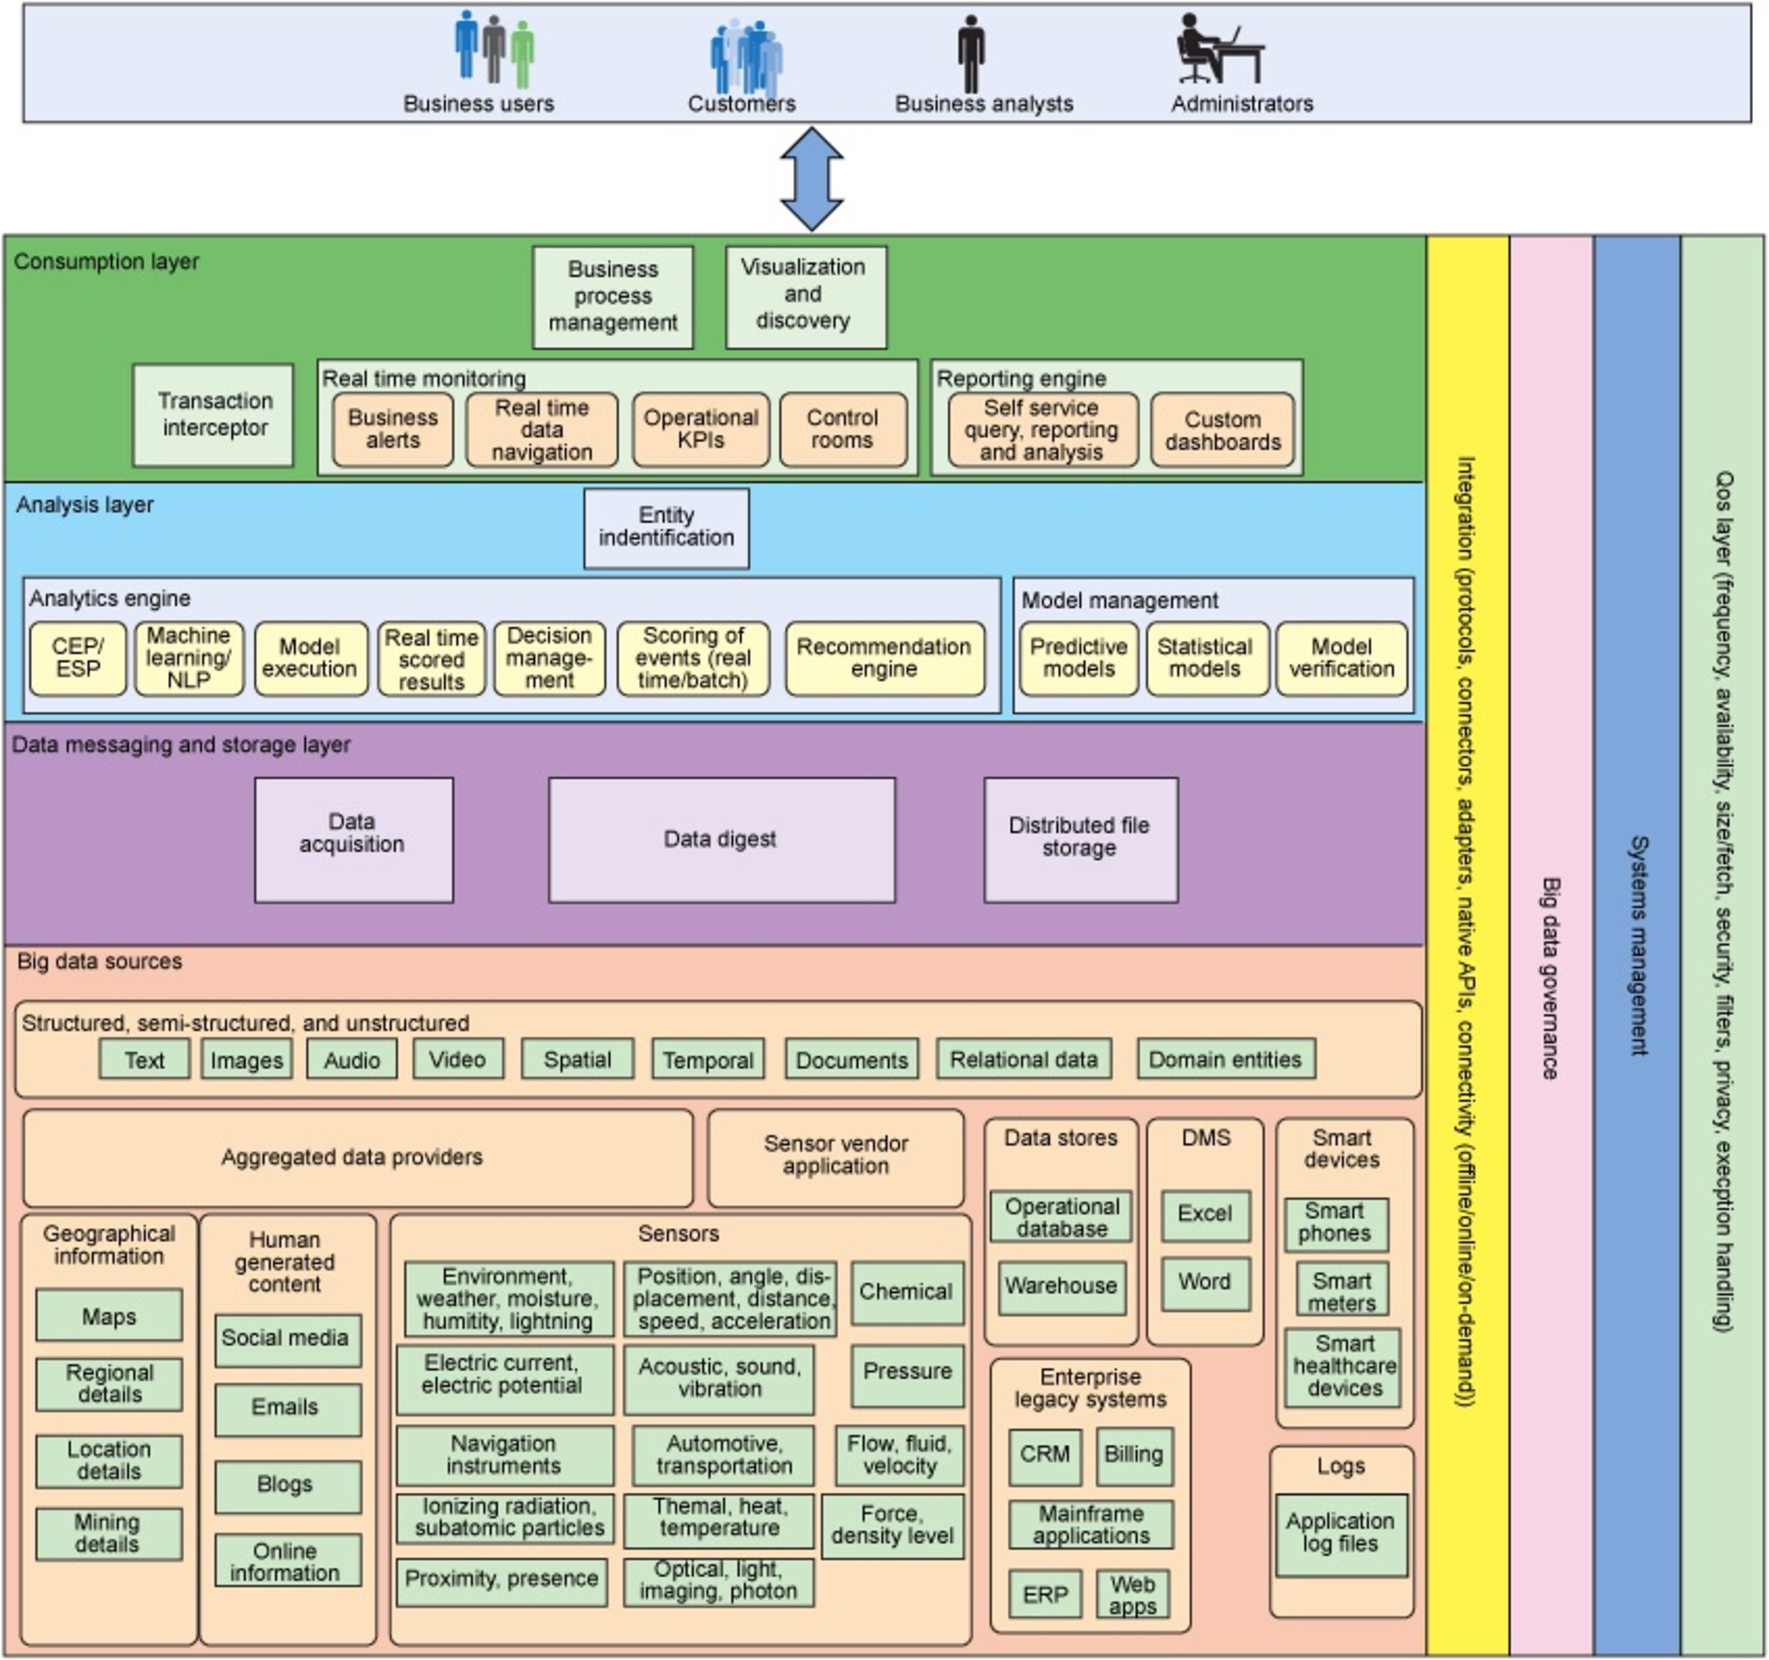
\includegraphics[height=7.5in, width=7.5in]{images/BigDataArchitecture.pdf}
\caption{Typical Big Data Architecture}
\end{figure}
 
\section{Drones and AI for Security}
Drones(Unmanned Aerial Vehicles) provide the ideal solution to the problems and limitations faced by Contemporary surveillance methods. Unlike a mounted camera, which is fixed on a designated area, drones are mobile and should be able to provide 360 degrees field view.Drones equipped with AI systems should be able to provide real-time insights for better decision making.Drone surveillance provides a lot of other key advantages like

\begin{itemize}
 \item Drone planes can enter narrow and confined spaces
 \item produce minimal noise
 \item  can be equipped with night vision cameras and thermal sensors
\end{itemize}
\subsection{Proposed Design for Drone Security System}
With the help of NVIDIA's Jetson TX2 platform it is possible to power drones with good Artificial Intelligence(AI).Drones with the TX2, FlytOS RealTime Object Detection solution can operate two cameras simultaneously.The Jetson platform making AI at the edge of the network, rather than in the cloud. Pre-trained model of a region  based convolutional neural network (R-CNN) deployed on the Nvidia  TX2  helps in recognizing and localizing objects like persons,cars, bikes etc.
  \begin{itemize}
    \item Micro Drone
    \item NVIDIA's Jetson TX2 platform 
    \item FlytOS RealTime
    \item NVIDIA TensorRT or Google's Tensor flow - high performance deep learning library
 \end{itemize}

\section{Community/Regional Security}

\section{Extended Regional Security}

\section{Conclusions}
In the today's technology world, drones are becoming more familiar in the main stream life activities such as recreational, spy cameras by authorities, home delivery of goods etc.

By making cameras movable across the house and outside and process the data as humans do and take decisions of alerting or informing to the right people is the key concept of this paper.This system to be functional, the following technologies needed:

\begin{itemize}
  
\item Micro drones with audio and video sensors

\item Facial recognition and mapping through video analytics to recognize people
	
\item Natural language processing (NLP) to recognize family members, friends and strangers

\item Machine learning algorithms to understand family members habits and behaviors

\item Interfacing with email servers, phone, text message servers

\end{itemize}

\begin{acks}
The authors would like to thank professor Gregor von Laszewski and his team for providing LaTex templates
\end{acks}

\bibliographystyle{ACM-Reference-Format}
\bibliography{report} 

\end{document}
